\begin{frame}[c] \frametitle{ Main Example: cooperative robots }
	\begin{figure}
		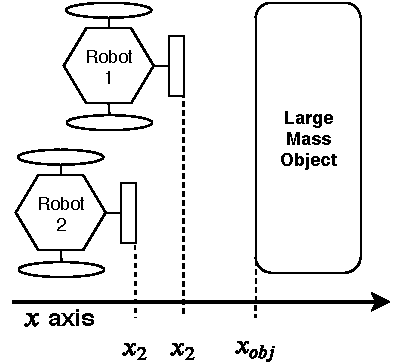
\includegraphics[width=0.45\textwidth]{./fig/diagrams/robots_diagram.pdf}
		\caption{A modified system presented in \footfullcite{chaimowicz2003hybrid}}
	\end{figure}
\end{frame}

\begin{frame}[c] \frametitle{ HIOA Model of cooperative robots }
	\begin{figure}
		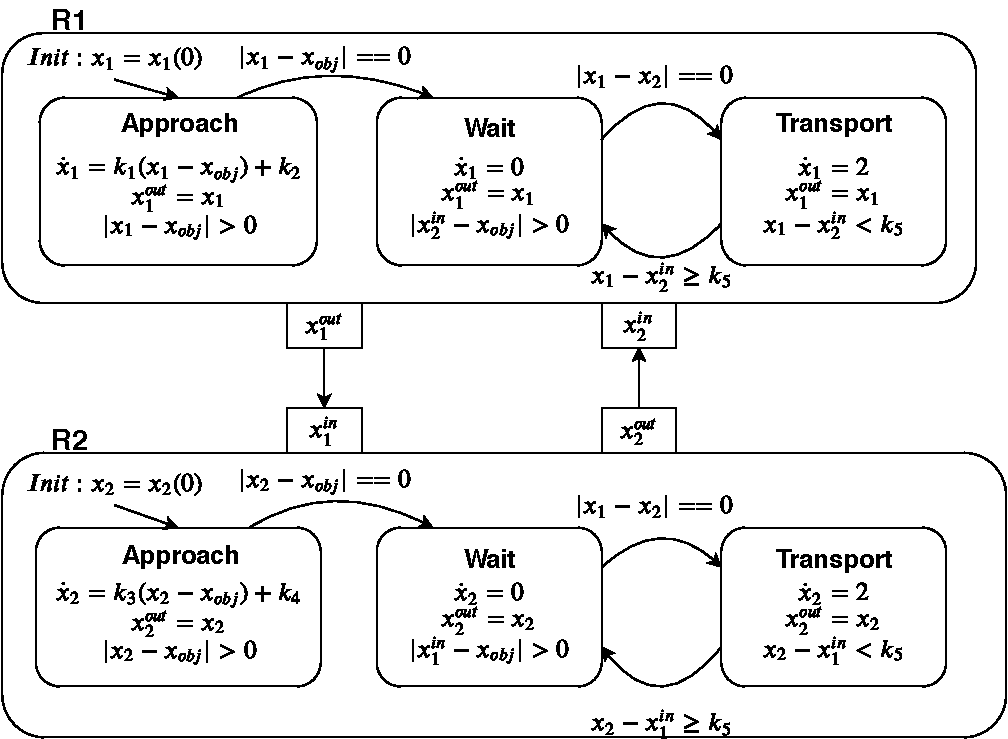
\includegraphics[width=0.7\textwidth]{./fig/diagrams/robots_ha.pdf}
		\caption{Hybrid automata model of cooperative robots. $k_1, k_2, k_3, k_4, k_5$, and $x_{obj}$ are constants. }
	\end{figure}
\end{frame}

\begin{frame}[c] \frametitle{ Other Example: Steeringwheel }
	\begin{figure}
		\centering
		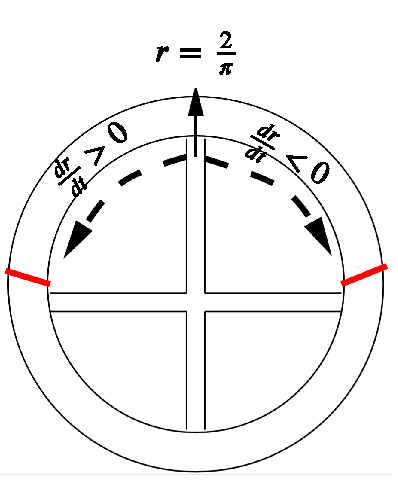
\includegraphics[width=0.4\textwidth]{./fig/diagrams/steeringwheel.pdf}
		\caption{Steeringwheel example in \footfullcite{ro2019compositional}}
	\end{figure}
\end{frame}

\begin{frame}[c] \frametitle{ Other Example: Two-tank }
	\begin{figure}
	\centering
	\begin{subfigure}{.4\textwidth}
	  \centering
	  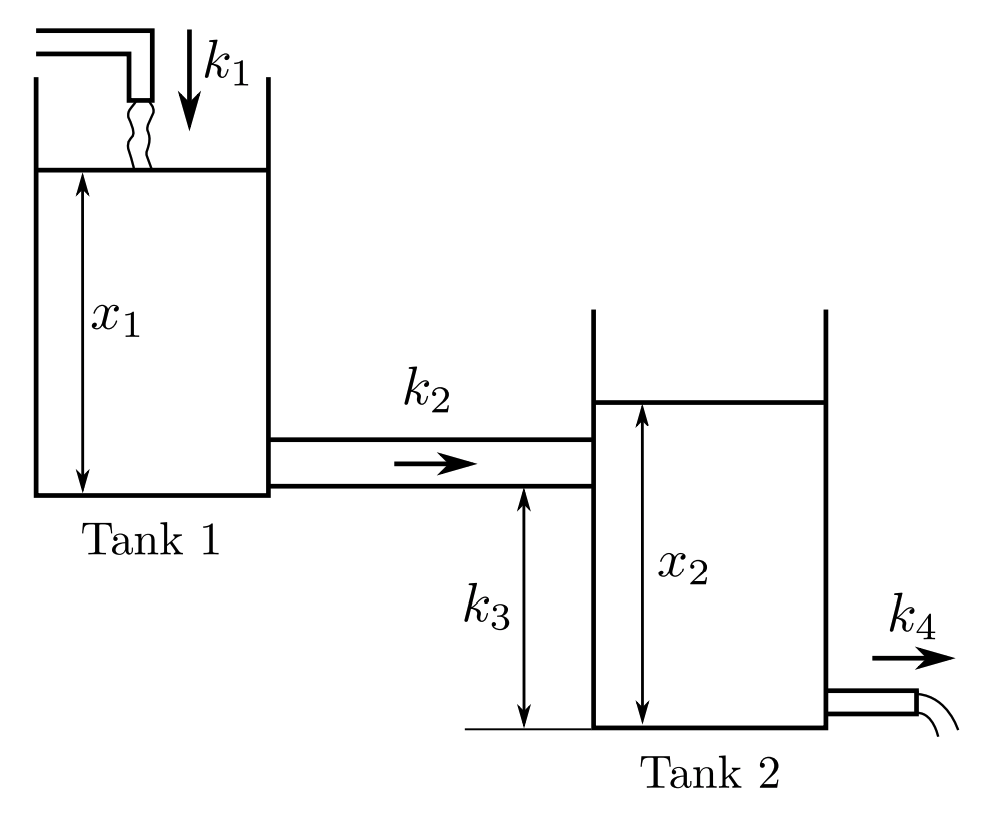
\includegraphics[width=0.8\textwidth]{./fig/diagrams/two-tank-diagram.png}
	  \caption{Physical setup}
	\end{subfigure}%
	\begin{subfigure}{.6\textwidth}
	  \centering
	  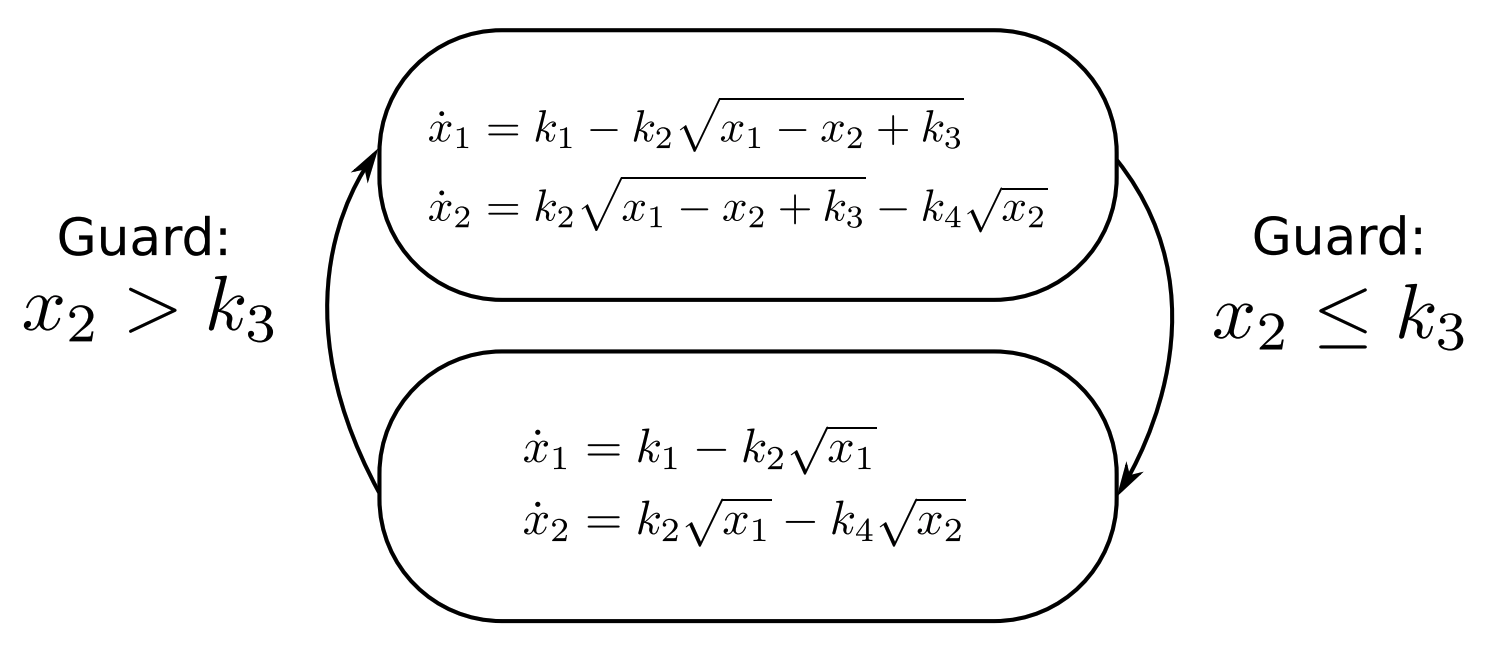
\includegraphics[width=1\linewidth]{./fig/diagrams/two-tank-ha.png}
	  \caption{A single hybrid automaton model}
	\end{subfigure}
	\caption{Two-tank example used in \footfullcite{navarro2016deadness}}
	\label{fig:test}
	\end{figure}
\end{frame}



